\chapter{L'ordinateur et les langages}
	\section{Systèmes informatique}
		\subsection{Traitement automatique d'une information pré enregistrée}
			\subsubsection{Information}
				\begin{itemize}
					\item[\textbullet] Concept abstrait à coder sous forme symbolique
				\end{itemize}
			\subsubsection{Traitement de l'information}	
				\begin{itemize}
					\item[\textbullet] Symboles codés transofmrés en d'autres symboles codés
				\end{itemize}
			\subsubsection{Automatisation}
				\begin{itemize}
					\item[\textbullet] Algorithme
				\end{itemize}
	\section{L'ordinateur}
		\subsection{Composantes}
			\subsubsection{Traitements}
				\begin{itemize}
					\item[\textbullet] Circuits élétroniques en tout ou rien
					\item[\textbullet] Actions de base: additionner, comparer, mémoriser, ...
				\end{itemize}
			\subsubsection{Mémoire}
				\begin{itemize}
					\item[\textbullet] Recevoir, conserver, restituer
					\item[\textbullet] Mémoire principale (très rapide)
					\item[\textbullet] Mémoire secondaire (très grosse capacité)
				\end{itemize}
			\subsubsection{Organes d'accès}
				\begin{itemize}
					\item[\textbullet] Communication avec l'extérieur
					\item[\textbullet] Entrée : clavier, souris, lecteurs, ...
					\item[\textbullet] Sortie: écran, imprimante, ...
				\end{itemize}
			\subsubsection{Fonctionnement}
				\includegraphics[width=445pt]{fonctionnement_ordi.eps}
			\subsubsection{Langages}
				\begin{itemize}
					\item[\textbullet] Langage Interne
					\begin{itemize}	
						\item Langage machine lié au matériel	
					\end{itemize}
					\item[\textbullet] Langages externes
						\begin{itemize}	
							\item Langages d'application
							\begin{itemize}
								\item[\textbullet] de haut niveau
								\item d'Assemblage
							\end{itemize}
							\item Langages de commande
							\begin{itemize}
								\item Éxécution de programmes 
								\item Manipulation de fichiers 
							\end{itemize}
						\end{itemize}
					\item[\textbullet] Transformation d'un langage externe en langage interne
						\begin{itemize}
							\item Interprétation
							\item Traduction : compilation ou assemblage
						\end{itemize}
						
				\end{itemize}
	\section{Architecture en couche des ordinateurs}
		\subsection{Conception descendante}
			\subsubsection{Similaire aux affinages en algorithmique}
		\subsection{Machine virtuelle}
			\subsubsection{Machine physique + logiciel}
		\subsection{Ordinateur consitué de trois couches}
			\subsubsection{Couche langage externe}
				\begin{itemize}
					\item [\textbullet] Vue par le programmeur d'application
				\end{itemize}
			\subsubsection{Couche machine}
				\begin{itemize}
					\item [\textbullet] Vue par le programmeur système 
				\end{itemize}
			\subsubsection{Couche physique}
				\begin{itemize}
					\item [\textbullet]Vue par le concepteur de machines 
				\end{itemize}
		\subsection{Entouré de deux autres couches}
	\section{Couche langage externe}
		\subsection{Programmes utilisateurs traduits à ce niveau}
			\begin{itemize}
				\item[\textbullet]Compilation ou assemblage
				\item[\textbullet]Édition de liens
			\end{itemize}
			
		\subsection{Problème de portabilité : trois solutions}
			\subsubsection{Langage de programmation universel}
				\begin{itemize}
					\item[\textbullet]Exemple: Ada
				\end{itemize}
			\subsubsection{Couche machine unique}
				\begin{itemize}
					\item[\textbullet] Exemple: Compatible PC
				\end{itemize}
			\subsubsection{Machine virtuelle}
				\begin{itemize}
					\item[\textbullet] Exemple: Java Virtual Machine (JVM) 
				\end{itemize}
				
		
	\section{Couche machine}
		\subsection{Décomposée en trois niveaux}
	\section{Processeur central (CPU)}
		\subsection{Aussi appellé microprocesseur}
		\subsection{Constitué de deux parties}
	\section{Processeur d'instructions}
		\subsection{Prélever l'instruction courante}
		\subsection{L'éxécuter}
		\subsection{Passer à l'instruction suivante}
	\section{Mémoire principale}
		\subsection{Constitué de cellules ou mots mémoire}
		\subsection{Un mot est constitué d'octet(s)}
		\subsection{Capacité de quelques kibioctets (Kio) à quelques gibioctets (Gio)}
		\subsection{Temps d'accès uniforme entre $1$ et $250 ns$}
		\subsection{Deux catégories}
	\section{Mémoire secondaire}
	\section{Niveau composants életroniques}
	\section{Niveau composants logiques}
	\section{Niveau circuits logiques}
	\section{Information}
	\section{Données}
	\section{Langage}
	\section{Construction d'un langage}
	\section{Puissance lexicographique}
	\section{Ordre lexicographique}
	\section{Assignation sémantique}
	\section{Codification}
	\section{Langage binaire}
	\section{Exemple de langage binaire}
		\subsection{Format fixe $=3$}
		\subsection{Format variable $\le 3$}
	\section{Représentation des éléments informationnels}
	\section{Représentation positionnée}
	\section{Représentation codifiée}
	\section{Utilisation des deux représentations}
	\section{Exemple d'un organe de calcul}
	\section{Utilisation d'un décodeur}
	\section{Représentation binaire d'un langage externe}
	\section{Codage de l'alphabet}
	\section{Code ISO 8859}
	\section{Code ISO 8859-1 (latin-1)}
	\section{Code iso 8859-15 (latin-9)}
	\section{Unicode}
	\section{UTF-8}
	\section{Contrôle de l'information}
	\section{Contrôle de Hamming}
	\section{Contrôle de Hamming + parité}
			

